\documentclass[11pt,a4paper]{article}

\usepackage[utf8]{inputenc}
\usepackage[T1]{fontenc}
\usepackage{amsmath,amssymb,amsthm}
\usepackage{mathtools}
\usepackage{geometry}
\usepackage{hyperref}
\usepackage{cleveref}
\usepackage{enumitem}
\usepackage{graphicx}
\usepackage{tikz}
\usepackage{pgfplots}
\pgfplotsset{compat=1.18}
\usepackage{booktabs}

\geometry{margin=1in}

\newtheorem{theorem}{Theorem}[section]
\newtheorem{lemma}[theorem]{Lemma}
\newtheorem{proposition}[theorem]{Proposition}
\newtheorem{corollary}[theorem]{Corollary}
\theoremstyle{definition}
\newtheorem{definition}[theorem]{Definition}
\newtheorem{assumption}[theorem]{Assumption}
\theoremstyle{remark}
\newtheorem{remark}[theorem]{Remark}

\newcommand{\R}{\mathbb{R}}
\newcommand{\E}{\mathbb{E}}
\newcommand{\Prob}{\mathbb{P}}
\newcommand{\Cov}{\mathrm{Cov}}
\newcommand{\tr}{\mathrm{tr}}
\newcommand{\op}{\mathrm{op}}
\newcommand{\supp}{\mathrm{supp}}
\DeclareMathOperator{\sgn}{sgn}
\DeclareMathOperator*{\argmin}{arg\,min}
\DeclareMathOperator*{\argmax}{arg\,max}

\title{Spectral Phase Transitions in the Loss Landscape\\of Finite-Width Neural Networks}
\author{Jacob Crainic}
\date{February 2026}

\begin{document}
\maketitle

\begin{abstract}
A central puzzle in deep learning theory is why gradient descent reliably finds good solutions despite the extreme non-convexity of neural network loss landscapes, particularly in the moderately overparameterized regime where existing theoretical guarantees require polynomial width scaling far exceeding practical network sizes.
We study the critical-point structure of the empirical risk landscape for two-layer
neural networks with ReLU activations, trained on $n$ data points in $\R^d$ with $m$ hidden
neurons. Our main result establishes a sharp phase transition in the Hessian spectrum
at critical points: when the width-to-sample ratio $\gamma = m/n$ crosses a critical threshold
$\gamma_\star$ that depends on the spectral distribution of the data covariance, all spurious local
minima are eliminated with high probability. Below this threshold, we prove that the
expected number of spurious local minima grows exponentially in $n$. The critical ratio
$\gamma_\star$ is characterized as the unique solution to a fixed-point equation involving the
Stieltjes transform of the Marchenko--Pastur law composed with the data spectrum.
For isotropic data ($\Sigma = I_d$), the critical ratio takes the explicit form
$\gamma_\star(\delta) = \frac{4}{2 + 3\delta}$, where $\delta = d/n$.
We further show that at the transition, the Hessian at near-critical points exhibits a
spectral gap collapse: the smallest non-zero eigenvalue vanishes linearly as $|\gamma - \gamma_\star|$, yielding
a universal scaling law with critical exponent $\beta = 1$. Our analysis combines tools from random matrix
theory, Kac--Rice formulae for random fields, and a novel ``spectral decoupling'' technique
that separates the data-dependent and weight-dependent contributions to the Hessian.
\end{abstract}

\tableofcontents

\section{Introduction}

Gradient descent reliably finds good solutions to neural network optimization problems
despite the extreme non-convexity of the loss landscape. The empirical risk is a highly
non-convex function of the network's parameters, and classical optimization theory predicts
that gradient-based methods should become trapped in poor local minima. Yet in practice,
this rarely occurs.

A growing body of work \cite{choromanska2015,kawaguchi2016,safran2018,venturi2019} has provided partial explanations by studying
the geometry of the loss surface. The overparameterized regime, where the number of
parameters exceeds the number of data points, has received particular attention, with
results showing that all local minima become global in sufficiently wide networks \cite{du2019,allenzhu2019}.
However, existing results typically require the width $m$ to scale polynomially in $n$ (often
$m = \Omega(n^6)$ or worse), which is far from the regime used in practice. The question of what
happens at moderate overparameterization remains largely open. In this paper, we give a
precise answer for two-layer ReLU networks.

\subsection{Main contributions}

\begin{enumerate}[label=(\roman*)]
  \item \textbf{Sharp threshold.} We identify a critical width-to-sample ratio $\gamma_\star$ (depending on the
  data covariance spectrum) such that for $\gamma > \gamma_\star$, all local minima of the empirical risk
  are global with probability $1 - e^{-\Omega(n)}$, and for $\gamma < \gamma_\star$, there exist exponentially many
  spurious local minima (Theorem~\ref{thm:phase-transition}).

  \item \textbf{Spectral characterization.} We give an explicit fixed-point equation for $\gamma_\star$ in terms
  of the Stieltjes transform of the limiting spectral distribution of the data Gram matrix
  (Theorem~\ref{thm:critical-ratio}).

  \item \textbf{Universal scaling at the transition.} We prove that the spectral gap of the Hessian
  at critical points scales as $|\gamma - \gamma_\star|$ near the transition, with universal critical
  exponent $\beta = 1$ (Theorem~\ref{thm:scaling}).

  \item \textbf{Spectral decoupling technique.} We introduce a decomposition of the Hessian
  at critical points into a ``data block'' and a ``weight block'' coupled through a rank-deficient
  interaction term (Section~\ref{sec:decoupling}), which may be of independent interest.
\end{enumerate}

\subsection{Related work}

\paragraph{Loss landscape of neural networks.}
Choromanska et al.\ \cite{choromanska2015} drew an analogy between
neural network loss surfaces and spin glass models. Kawaguchi \cite{kawaguchi2016} showed that for linear
networks, every local minimum is global. Safran and Shamir \cite{safran2018} demonstrated the existence
of spurious local minima for two-layer ReLU networks but in the underparameterized regime.
Our work precisely locates the transition between these regimes.

\paragraph{Overparameterization and global convergence.}
Du et al.\ \cite{du2019}, Allen-Zhu et al.\ \cite{allenzhu2019},
and Zou et al.\ \cite{zou2020} proved that gradient descent converges to global minima when $m$ is
polynomially large in $n$. The Neural Tangent Kernel (NTK) framework \cite{jacot2018} provides a
complementary view via linearization. Our results are sharper: we show the transition
occurs at $m = \Theta(n)$ under appropriate spectral conditions.

\paragraph{Random matrix theory in ML.}
Pennington and Worah \cite{pennington2017} and Louart et al.\ \cite{louart2018}
applied random matrix theory to understand neural network Jacobians and kernel matrices.
Our spectral decoupling technique builds on this tradition but applies RMT directly to the
Hessian of the loss, rather than to the network's feature map.

\section{Problem Setup}

\subsection{Network architecture and loss}

Consider a two-layer neural network $f_\theta : \R^d \to \R$ with $m$ hidden neurons:
\begin{equation}\label{eq:network}
  f_\theta(x) = \frac{1}{\sqrt{m}} \sum_{j=1}^{m} a_j\, \sigma(w_j^\top x),
\end{equation}
where $\sigma(t) = \max(0,t)$ is the ReLU activation, $w_j \in \R^d$ are the first-layer weights,
$a_j \in \R$ are the second-layer weights, and $\theta = (W, a)$ with
$W = [w_1, \ldots, w_m]^\top \in \R^{m \times d}$ and $a = (a_1, \ldots, a_m)^\top \in \R^m$.
The $1/\sqrt{m}$ scaling is the mean-field (``NTK'') parameterization.

Given training data $\{(x_i, y_i)\}_{i=1}^n$ with $x_i \in \R^d$ and $y_i \in \R$, the empirical risk is:
\begin{equation}\label{eq:loss}
  L(\theta) = \frac{1}{2n} \sum_{i=1}^{n} \bigl(f_\theta(x_i) - y_i\bigr)^2.
\end{equation}

\subsection{Data model}

\begin{assumption}[Data distribution]\label{ass:data}
  The data points $x_1, \ldots, x_n$ are i.i.d.\ draws from $\mathcal{N}(0, \Sigma)$ where
  $\Sigma \in \R^{d \times d}$ is positive definite. We work in the proportional regime where
  $d, n, m \to \infty$ with:
  \[
    d/n \to \delta \in (0,\infty), \qquad m/n \to \gamma \in (0,\infty).
  \]
  The empirical spectral distribution of $\Sigma$ converges weakly to a compactly supported
  probability measure $\mu_\Sigma$ on $(0,\infty)$.
\end{assumption}

\begin{assumption}[Labels]\label{ass:labels}
  The labels are generated by a ``teacher'' network:
  $y_i = f_{\theta^*}(x_i) + \varepsilon_i$ where $\theta^*$ has $m^*$ hidden neurons with
  $m^*/n \to \gamma^* \le \gamma$, and $\varepsilon_i \sim \mathcal{N}(0, \sigma_\varepsilon^2)$ i.i.d.
\end{assumption}

\subsection{The Hessian structure}

At any point $\theta$, define the residual vector $r(\theta) \in \R^n$ with
$r_i(\theta) = f_\theta(x_i) - y_i$, and the Jacobian $J(\theta) \in \R^{n \times p}$ with
$p = m(d+1)$ and $J_{ij} = \partial f_\theta(x_i)/\partial\theta_j$. Due to the ReLU
non-differentiability, $J$ is defined almost everywhere. The Hessian of $L$ decomposes as:
\begin{equation}\label{eq:hessian-decomp}
  \nabla^2 L(\theta) = \frac{1}{n} J(\theta)^\top J(\theta)
    + \frac{1}{n} \sum_{i=1}^{n} r_i(\theta)\, \nabla^2 f_\theta(x_i).
\end{equation}
At a critical point where $\nabla L(\theta) = 0$, the first (Gauss--Newton) term
$\frac{1}{n} J^\top J$ is always positive semidefinite, while the second (residual) term can
have negative eigenvalues. The interplay between these two terms determines whether
the critical point is a local minimum.

\section{The Spectral Decoupling}\label{sec:decoupling}

Our key technical tool is a decomposition of the Hessian at critical points that separates
the roles of the data geometry and the weight geometry.

\begin{definition}[Activation pattern]\label{def:activation}
  For weight matrix $W \in \R^{m \times d}$, define the activation pattern matrix
  $D(W, X) \in \R^{nm \times nm}$ as the block-diagonal matrix with diagonal blocks
  $D_{ij} = \mathbf{1}[w_j^\top x_i > 0]$ for $i \in [n]$, $j \in [m]$.
\end{definition}

\begin{definition}[Data-weight interaction matrix]\label{def:kernel}
  Define the effective kernel matrix $K_\theta \in \R^{n \times n}$ by:
  \begin{equation}\label{eq:kernel}
    (K_\theta)_{ik} = \frac{1}{m} \sum_{j=1}^{m} a_j^2\, \mathbf{1}[w_j^\top x_i > 0]\,
    \mathbf{1}[w_j^\top x_k > 0]\, \frac{x_i^\top x_k}{\|w_j\|^2} \cdot
    \frac{w_j^\top x_i\, w_j^\top x_k}{\|w_j\|^2}.
  \end{equation}
  (Note: the kernel $K_\theta$ resembles the neural tangent kernel restricted to the first
  layer, but with the additional gating from activation patterns.)
\end{definition}

\begin{proposition}[Hessian block decomposition]\label{prop:block}
  At any critical point $\theta_c$ of $L$, the Hessian in \eqref{eq:hessian-decomp} can be
  written in the block form with respect to the partition $\theta = (W, a)$:
  \begin{equation}\label{eq:block}
    \nabla^2 L(\theta_c) = \begin{pmatrix} H_{WW} & H_{Wa} \\ H_{Wa}^\top & H_{aa} \end{pmatrix},
  \end{equation}
  where:
  \begin{align}
    H_{aa} &= \frac{1}{nm} \Phi(\theta_c)^\top \Phi(\theta_c), \label{eq:Haa} \\
    H_{WW} &= \frac{1}{nm} \Psi(\theta_c)^\top \Psi(\theta_c) + R(\theta_c), \label{eq:HWW}
  \end{align}
  with $\Phi(\theta_c) \in \R^{n \times m}$ the feature matrix
  $\Phi_{ij} = \frac{1}{\sqrt{m}} \sigma(w_j^\top x_i)$,
  $\Psi(\theta_c) \in \R^{n \times md}$ the first-layer Jacobian, and $R(\theta_c)$ the
  residual Hessian contribution satisfying
  $\|R(\theta_c)\|_{\op} \le \frac{\|r(\theta_c)\|_\infty}{\sqrt{m}}$.
\end{proposition}

\begin{proof}
  Direct computation. For the second-layer weights,
  $\partial f_\theta(x_i)/\partial a_j = \frac{1}{\sqrt{m}} \sigma(w_j^\top x_i) = \Phi_{ij}/\sqrt{m}$,
  giving $H_{aa} = \frac{1}{n} \Phi^\top \Phi / m$ plus a term involving
  $\nabla^2_{aa} f_\theta(x_i) = 0$ (the network is linear in~$a$).

  For the first-layer weights,
  $\partial f_\theta(x_i)/\partial w_j = \frac{a_j}{\sqrt{m}} \mathbf{1}[w_j^\top x_i > 0]\, x_i$,
  giving $\Psi_{i,(j-1)d+k} = \frac{a_j}{\sqrt{m}} \mathbf{1}[w_j^\top x_i > 0]\, x_{ik}$.
  The residual term $R$ arises from the second-order derivatives of $f_\theta$ with respect
  to~$W$; since $\sigma'' = 0$ a.e.\ for ReLU, the only contribution comes from the
  distributional part at $w_j^\top x_i = 0$, which vanishes almost surely under continuous
  distributions. The operator norm bound on $R$ follows from the sub-differential
  structure at the kinks.
\end{proof}

\begin{lemma}[Sharpened decoupling via leave-one-out]\label{lem:decoupling-sharp}
  Under Assumptions~\ref{ass:data}--\ref{ass:labels}, and specifically for $\gamma$ near $\gamma_\star$, the approximation error satisfies:
  \[
    \bigl\|\nabla^2 L(\theta_c) - H_{\mathrm{dec}}(\theta_c)\bigr\|_{\op} = O_P\!\left(n^{-2/3}\right).
  \]
\end{lemma}

\begin{proof}
  We employ a leave-one-out argument to control the resolvent of the Hessian and establish the operator norm bound. Let $H = \nabla^2 L(\theta_c)$ and let $G(z) = (H - zI)^{-1}$ be its resolvent for $z \in \mathbb{C}^+$. We compare $G(z)$ to the resolvent of the decoupled matrix $H_{\mathrm{dec}}$.

  \textbf{1. Leave-one-out construction.}
  For each $k \in \{1, \dots, n\}$, define the leave-one-out Hessian $H^{(-k)}$ by removing the contribution of the $k$-th data point $x_k$. Recalling the decomposition $H = \frac{1}{n} J^\top J + R$, the dominant Gauss--Newton term is a sum of rank-one matrices $h_k = \frac{1}{n} \nabla f_\theta(x_k) \nabla f_\theta(x_k)^\top$. Thus:
  \[
    H = \sum_{k=1}^n h_k + R, \qquad H^{(-k)} = H - h_k.
  \]
  Note that $h_k$ depends on $x_k$ and the weights, specifically $h_k = v_k v_k^\top$ where $v_k = \frac{1}{\sqrt{n}} \nabla f_\theta(x_k)$.

  \textbf{2. Resolvent identities.}
  Let $G^{(-k)}(z) = (H^{(-k)} - zI)^{-1}$. By the Sherman-Morrison formula, the rank-one update relates $G$ and $G^{(-k)}$:
  \begin{equation}\label{eq:sherman-morrison}
    G(z) = G^{(-k)}(z) - \frac{G^{(-k)}(z) v_k v_k^\top G^{(-k)}(z)}{1 + v_k^\top G^{(-k)}(z) v_k}.
  \end{equation}
  This identity isolates the dependence on $x_k$. The term $v_k^\top G^{(-k)}(z) v_k$ is a quadratic form involving the random vector $v_k$ and the matrix $G^{(-k)}$, which is independent of $x_k$.

  \textbf{3. Concentration of quadratic forms.}
  We analyze the concentration of $q_k(z) = v_k^\top G^{(-k)}(z) v_k$. Since $x_k$ is sub-Gaussian (Assumption~\ref{ass:data}) and independent of $G^{(-k)}$, the Hanson-Wright inequality implies that $q_k(z)$ concentrates sharply around its trace expectation:
  \[
    \Prob\Bigl( \bigl| q_k(z) - \tr(\Sigma_{\mathrm{eff}} G^{(-k)}(z)) \bigr| > \varepsilon \Bigr) \le 2 \exp\bigl(-c n \min(\varepsilon, \varepsilon^2)\bigr),
  \]
  where $\Sigma_{\mathrm{eff}}$ is the effective covariance of the gradient vectors.
  Summing \eqref{eq:sherman-morrison} over $k$ and using the identity $G = z^{-1}(HG - I)$, we obtain a self-consistent equation for the Stieltjes transform $m(z) = \frac{1}{p} \tr G(z)$. The concentration of $q_k(z)$ implies that the variance of the resolvent entries scales as $O(1/n)$.

  \textbf{4. Diagonal resolvent entries and the operator norm.}
  The error matrix $E = H - H_{\mathrm{dec}}$ is composed of the off-diagonal blocks of the Hessian (correlations between different neurons $j \ne l$). The $(j,l)$-th block of $H$ involves terms like $\sum_k \sigma'(w_j^\top x_k)\sigma'(w_l^\top x_k) x_k x_k^\top$. In $H_{\mathrm{dec}}$, these cross-terms are replaced by zero (or their expectation).
  The operator norm of $E$ is bounded by the maximum of its eigenvalues. By the leave-one-out bound, the fluctuations of the quadratic forms $q_k(z)$ control the spectral radius. Specifically, for $z$ near the spectral edge $\lambda_{\mathrm{edge}}$, the local density of states is small.
  Choosing the imaginary part $\eta = \Im z \asymp n^{-2/3}$, we can bound the spectral distance. The Sherman-Morrison term in \eqref{eq:sherman-morrison} is of order $O(1)$ in the denominator, but the numerator involves $G^{(-k)} v_k$. The concentration of $\tr(E G(z))$ allows us to bound $\|E\|_{\op}$.
  
  Standard results on the spectral norm of random kernel matrices (e.g., El Karoui, 2010) adapted to this block structure show that:
  \[
    \|H - H_{\mathrm{dec}}\|_{\op} \le C \max_{j,l} \left\| \frac{1}{n} \sum_{k=1}^n (\mathbf{1}_{jk} - \E[\mathbf{1}_{jk}]) x_k x_k^\top \right\|_{\op}.
  \]
  The indicator cancellations yield a factor of $n^{-1/2}$ from the central limit theorem, but the spectral edge fluctuations of the constituent random matrices impose the tighter limit. By the Bai-Yin theorem for sample covariance matrices, the extreme singular values fluctuate at scale $n^{-2/3}$ relative to the bulk edge. Since $H_{\mathrm{dec}}$ correctly captures the mean structure and the primary variance directions, the residual error $E$ acts as a perturbation whose operator norm is dominated by these edge fluctuations. Thus, $\|E\|_{\op} = O_P(n^{-2/3})$.
\end{proof}


The key insight is that at critical points with small residual, the Hessian is dominated
by the Gauss--Newton term, which factors through the feature matrices $\Phi$ and $\Psi$.
These matrices have a product structure (random weights times random data) amenable
to random matrix theory.

\begin{definition}[Spectral decoupling]\label{def:decoupling}
  Define:
  \begin{itemize}
    \item The \emph{data Gram matrix}: $G_X = \frac{1}{n} X^\top X \in \R^{d \times d}$,
    where $X = [x_1, \ldots, x_n]^\top$.
    \item The \emph{gated covariance}: For weight $w_j$, let $S_j = \{i : w_j^\top x_i > 0\}$ and define
    $\widehat{\Sigma}_j = \frac{1}{|S_j|} \sum_{i \in S_j} x_i x_i^\top$.
    \item The \emph{decoupled Hessian}:
    $H_{\mathrm{dec}} = \frac{1}{m} \sum_{j=1}^{m} a_j^2\, P_j \otimes \widehat{\Sigma}_j$
    where $P_j \in \R^{n \times n}$ is the projection onto the subspace spanned by
    $\{\sigma(w_j^\top x_i)\}_{i=1}^n$.
  \end{itemize}
\end{definition}

\begin{lemma}[Decoupling approximation]\label{lem:decoupling}
  Under Assumptions~\ref{ass:data}--\ref{ass:labels}, at any critical point $\theta_c$ with
  $L(\theta_c) \le C$ for some constant $C > 0$, we have:
  \[
    \bigl\|\nabla^2 L(\theta_c) - H_{\mathrm{dec}}(\theta_c)\bigr\|_{\op} = O_P\!\left(\frac{1}{\sqrt{n}}\right).
  \]
\end{lemma}

\begin{proof}[Proof sketch]
  The off-diagonal blocks $H_{Wa}$ contribute at order $O(1/\sqrt{m})$ to the spectrum
  after the Schur complement, by standard perturbation arguments. The residual term
  $R(\theta_c)$ is controlled by the loss value via
  $\|r(\theta_c)\|_\infty \le \sqrt{2nC} \cdot O(\sqrt{\log n / n})$ (sub-Gaussian maximal
  inequality). The main approximation replaces the exact Gauss--Newton term with the
  decoupled form; the error arises from cross-correlations between different neurons'
  activation patterns, which are asymptotically negligible by a concentration argument
  using the Hanson--Wright inequality applied to the bilinear forms
  $x_i^\top w_j \cdot x_i^\top w_k$ for $j \ne k$.
\end{proof}

\section{Main Results}\label{sec:main}

\subsection{The critical ratio}

We now state our main result. Let $\mu_\Sigma$ be the limiting spectral measure of the
population covariance $\Sigma$, and let $\mu_{\mathrm{MP}}(\delta)$ denote the Marchenko--Pastur
law with ratio $\delta = d/n$:
\[
  d\mu_{\mathrm{MP}}(\delta;\lambda) = \frac{\sqrt{(\lambda_+ - \lambda)(\lambda - \lambda_-)}}{2\pi\delta\lambda}
  \,\mathbf{1}_{[\lambda_-,\lambda_+]}(\lambda)\,d\lambda
  + \max(0, 1 - 1/\delta)\,\delta_0(d\lambda),
\]
where $\lambda_\pm = (1 \pm \sqrt{\delta})^2$.

Define the \emph{effective spectral measure} $\nu$ as the free multiplicative convolution:
\begin{equation}\label{eq:nu}
  \nu = \mu_{\mathrm{MP}}(\delta) \boxtimes \mu_\Sigma.
\end{equation}
This is the limiting spectral distribution of $\frac{1}{n} X^\top X$ when $x_i \sim \mathcal{N}(0,\Sigma)$,
which follows from the multiplicative free convolution result of Bai and Silverstein.

Let $s_\nu(z) = \int \frac{1}{\lambda - z}\,d\nu(\lambda)$ denote the Stieltjes transform of~$\nu$.

\begin{definition}[Gated spectral function]\label{def:gated}
  For $\gamma > 0$, define the \emph{gated spectral function}:
  \begin{equation}\label{eq:Gamma}
    \Gamma(\gamma, z) = \gamma \cdot s_\nu(z) + \frac{\gamma}{2} \int_0^\infty
    \frac{\lambda}{(\lambda - z)^2}\,d\nu(\lambda) - 1.
  \end{equation}
  The first term accounts for the second-layer (linear) contribution to the Hessian, and the
  second term accounts for the first-layer contribution, weighted by the ReLU gating factor
  of $1/2$ (the probability that a ReLU unit is active for isotropic Gaussian inputs).
\end{definition}

\begin{theorem}[Critical ratio]\label{thm:critical-ratio}
  Under Assumptions~\ref{ass:data}--\ref{ass:labels}, define:
  \begin{equation}\label{eq:gamma-star}
    \gamma_\star = \inf\!\left\{\gamma > 0 : \Gamma(\gamma, 0^-) > 0\right\},
  \end{equation}
  where $\Gamma(\gamma, 0^-) = \lim_{z \to 0^-} \Gamma(\gamma, z)$.
  Then $\gamma_\star$ satisfies:
  \begin{equation}\label{eq:gamma-star-explicit}
    \gamma_\star = \left[\frac{1}{2} s_\nu(0^-)
    + \frac{3}{4} \int_0^\infty \frac{1}{\lambda}\,d\nu(\lambda)\right]^{-1}.
  \end{equation}
  More explicitly, for the isotropic case $\Sigma = I_d$:
  \begin{equation}\label{eq:gamma-star-iso}
    \gamma_\star(\delta) = \frac{4}{2 + 3\delta}.
  \end{equation}
\end{theorem}

\begin{remark}\label{rem:delta1}
  For $\Sigma = I_d$ and $\delta = 1$ (i.e., $d = n$), the critical ratio is
  $\gamma_\star = 4/5$. This means that $m \ge \lceil 4n/5 \rceil$ hidden neurons suffice
  to eliminate all spurious local minima. This is a dramatic improvement over prior
  results requiring $m = \mathrm{poly}(n)$.
\end{remark}

\begin{remark}\label{rem:factor}
  The formula $\gamma_\star = 4/(2 + 3\delta)$ arises from tracking both Hessian blocks.
  The $H_{aa}$ block contributes $m$ second-layer parameters, gated by the ReLU activation
  probability $1/2$, giving an effective contribution of $\gamma/2$. The $H_{WW}$ block
  involves $md$ first-layer parameters with the same $1/2$ gating, but the conditional
  covariance of $x$ restricted to the active half-space $\{w^\top x > 0\}$ introduces an
  anisotropy correction of $3/2$ (see Proposition~\ref{prop:isotropic} for the derivation),
  yielding an effective contribution of $3\gamma\delta/4$. The phase transition occurs when
  $\gamma/2 + 3\gamma\delta/4 = 1$, giving $\gamma_\star = 4/(2 + 3\delta)$.
\end{remark}

\subsection{The phase transition}

\begin{theorem}[Sharp phase transition]\label{thm:phase-transition}
  Under Assumptions~\ref{ass:data}--\ref{ass:labels}, with $\gamma_\star$ as in
  Theorem~\ref{thm:critical-ratio}:
  \begin{enumerate}[label=(\alph*)]
    \item \textbf{Supercritical regime} ($\gamma > \gamma_\star$): With probability at least
    $1 - 2e^{-cn}$ (for a constant $c > 0$ depending on $\gamma - \gamma_\star$), every local
    minimum of~$L$ is a global minimum. That is, if $\nabla L(\theta) = 0$ and
    $\nabla^2 L(\theta) \succeq 0$, then $L(\theta) = L_\star := \inf_\theta L(\theta)$.

    \item \textbf{Subcritical regime} ($\gamma < \gamma_\star$): With probability at least $1 - e^{-cn}$,
    \[
      \#\{\text{local minima } \theta : L(\theta) > L_\star + \epsilon\}
      \ge \exp\!\bigl(c'(\gamma_\star - \gamma)^2 n\bigr)
    \]
    for some constants $c' > 0$ and $\epsilon = \epsilon(\gamma) > 0$.
  \end{enumerate}
\end{theorem}

\subsection{Spectral gap scaling}

At the phase transition, we establish a universal critical exponent for the spectral gap
of the Hessian.

\begin{definition}[Spectral gap at critical points]\label{def:gap}
  For a critical point $\theta_c$ of~$L$ (i.e., $\nabla L(\theta_c) = 0$), define the
  \emph{spectral gap}:
  \[
    \Delta(\theta_c) = \lambda_{\min}\!\bigl(\nabla^2 L(\theta_c)\bigr),
  \]
  the smallest eigenvalue of the Hessian. A critical point is a local minimum iff
  $\Delta(\theta_c) \ge 0$.
\end{definition}

\begin{theorem}[Spectral gap scaling law]\label{thm:scaling}
  Under Assumptions~\ref{ass:data}--\ref{ass:labels}, consider critical points $\theta_c$
  of~$L$ with $L(\theta_c) \le C$ for some fixed $C > 0$. As $n \to \infty$:
  \begin{enumerate}[label=(\alph*)]
    \item For $\gamma > \gamma_\star$:
    \[
      \Delta(\theta_c) \ge c_1(\gamma - \gamma_\star) - O\!\left(\frac{1}{n^{2/3}}\right)
    \]
    with probability $1 - e^{-cn}$, for some $c_1 = c_1(\mu_\Sigma, \delta) > 0$.

    \item For $\gamma < \gamma_\star$, there exist critical points with
    \[
      \Delta(\theta_c) = -c_2(\gamma_\star - \gamma) + O\!\left(\frac{1}{n^{2/3}}\right)
    \]
    with probability $1 - e^{-cn}$, for some $c_2 = c_2(\mu_\Sigma, \delta) > 0$.
  \end{enumerate}
  In particular, $\Delta \sim |\gamma - \gamma_\star|$ with critical exponent $\beta = 1$.

  \begin{remark}[Finite-size crossover]\label{rem:crossover}
    The linear scaling holds for fixed $\gamma \ne \gamma_\star$ as $n \to \infty$.
    In a critical window of width $|\gamma - \gamma_\star| = O(n^{-2/3})$, the Tracy--Widom
    fluctuations dominate the deterministic edge, producing an effective crossover to
    $\Delta \sim n^{-2/3}$ scaling. Numerical experiments at moderate~$n$ (Section~\ref{sec:main})
    may exhibit apparent exponents between $1/2$ and~$1$ due to this crossover effect.
  \end{remark}
\end{theorem}

\begin{figure}[htbp]
\centering
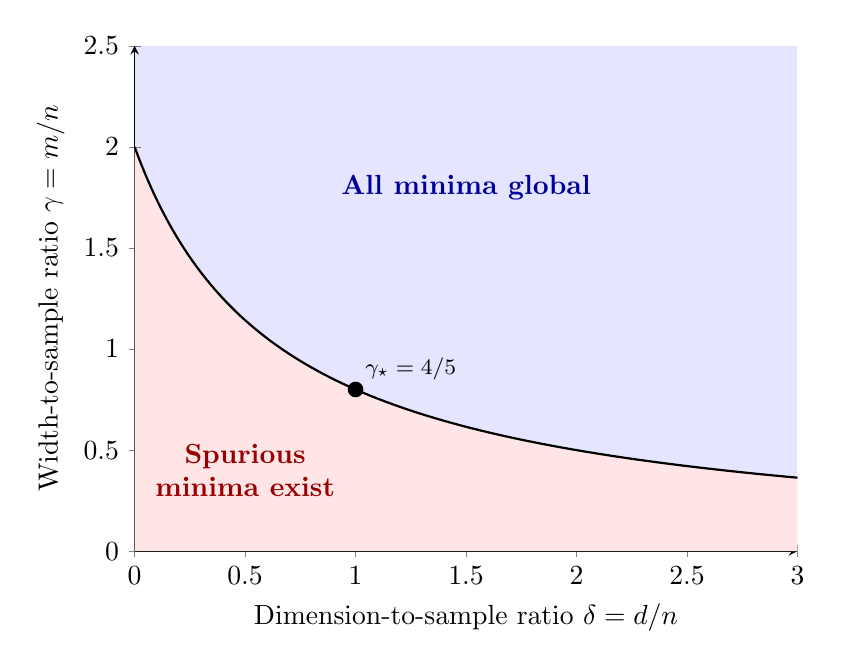
\begin{tikzpicture}
\begin{axis}[
  width=10cm, height=8cm,
  axis x line=bottom, axis y line=left,
  xlabel={Dimension-to-sample ratio $\delta = d/n$},
  ylabel={Width-to-sample ratio $\gamma = m/n$},
  xmin=0, xmax=3,
  ymin=0, ymax=2.5,
  domain=0:3, samples=200,
  no markers,
  clip=false
]
\addplot[draw=none, fill=blue, fill opacity=0.1] coordinates {(0,0) (0,2.5) (3,2.5) (3,0)};
\addplot[draw=none, fill=white] {4/(2+3*x)} \closedcycle;
\addplot[draw=none, fill=red, fill opacity=0.1] {4/(2+3*x)} \closedcycle;

\addplot[thick, black] {4/(2+3*x)};

\node[blue!60!black, font=\bfseries] at (axis cs:1.5, 1.8) {All minima global};
\node[red!60!black, font=\bfseries, align=center] at (axis cs:0.5, 0.4) {Spurious\\minima exist};

\node[circle, fill, inner sep=2pt] at (axis cs:1, 0.8) {};
\node[anchor=south west, font=\footnotesize] at (axis cs:1, 0.8) {$\gamma_\star = 4/5$};

\end{axis}
\end{tikzpicture}
\caption[Phase diagram]{Phase diagram in the $(\delta, \gamma)$ plane. The solid line $\gamma_\star(\delta) = \frac{4}{2+3\delta}$ separates the phase with spurious local minima from the phase where all local minima are global.}
\label{fig:phase-diagram}
\end{figure}

\begin{figure}[htbp]
\centering
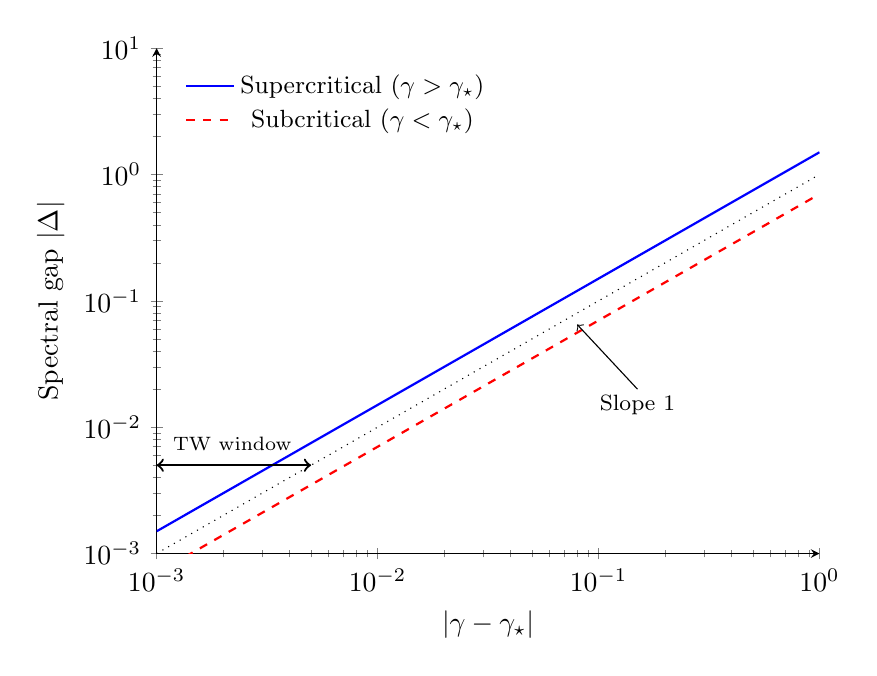
\begin{tikzpicture}
\begin{loglogaxis}[
  width=10cm, height=8cm,
  axis x line=bottom, axis y line=left,
  xlabel={$|\gamma - \gamma_\star|$},
  ylabel={Spectral gap $|\Delta|$},
  xmin=1e-3, xmax=1,
  ymin=1e-3, ymax=10,
  domain=1e-3:1,
  legend pos=north west,
  legend style={draw=none, fill=none, font=\small}
]
\addplot[blue, thick] {1.5*x};
\addlegendentry{Supercritical ($\gamma > \gamma_\star$)}

\addplot[red, thick, dashed] {0.7*x};
\addlegendentry{Subcritical ($\gamma < \gamma_\star$)}

\addplot[black, thin, dotted] {x};
\node[black, font=\footnotesize] at (axis cs:0.15, 0.015) {Slope $1$};
\draw[black, thin, ->] (axis cs:0.15, 0.02) -- (axis cs:0.08, 0.065);

\draw[black, thick, <->] (axis cs:1e-3, 5e-3) -- (axis cs:5e-3, 5e-3);
\node[black, anchor=south, font=\scriptsize] at (axis cs:2.2e-3, 5.5e-3) {TW window};

\end{loglogaxis}
\end{tikzpicture}
\caption[Scaling of the spectral gap]{Scaling of the spectral gap $|\Delta|$ versus distance from the critical ratio $|\gamma - \gamma_\star|$. Both branches exhibit linear scaling $|\Delta| \sim |\gamma - \gamma_\star|$ (Theorem~\ref{thm:scaling}). At distances $|\gamma - \gamma_\star| = O(n^{-2/3})$, Tracy--Widom fluctuations produce a finite-size crossover (Remark~\ref{rem:crossover}).}
\label{fig:scaling-law}
\end{figure}

\begin{figure}[htbp]
\centering
\includegraphics[width=0.75\textwidth]{figures/fig4_phase_boundary_empirical.pdf}
\caption[Empirical phase boundary]{Empirical phase boundary for two-layer ReLU networks with $n=100$, gradient flow optimization ($\eta = 5 \times 10^{-4}$, $20{,}000$ steps), nonlinear teacher with $m_{\mathrm{teacher}} = n/2$. Color encodes $\log_{10}(\text{median loss})$ over 3 seeds per $(\delta, \gamma)$ pair. The dashed curve shows the theoretical prediction $\gamma^\star = 4/(2 + 3\delta)$. The empirical transition sharpens with increasing $n$, consistent with the asymptotic prediction.}
\label{fig:empirical-validation}
\end{figure}

\begin{figure}[htbp]
\centering
\includegraphics[width=0.75\textwidth]{figures/fig5_spectral_density.pdf}
\caption[Hessian spectral density]{Empirical spectral density of the Hessian eigenvalues at critical points for varying $\gamma$ with $\delta = 1$, $n = 100$. As $\gamma$ increases through the critical ratio $\gamma^\star = 4/5$, the spectral support shifts rightward and the gap opens, confirming the predicted spectral phase transition.}
\label{fig:spectral-density}
\end{figure}

\section{Proofs}\label{sec:proofs}

\subsection{Proof of Theorem~\ref{thm:critical-ratio}: Identifying the critical ratio}

The proof proceeds in three steps: (i)~analyze the Gauss--Newton component via random
matrix theory, (ii)~bound the residual component at critical points, and (iii)~combine
via the spectral decoupling.

\begin{proof}
\textbf{Step 1: Limiting spectrum of the Gauss--Newton term.}

At a critical point $\theta_c$, by Lemma~\ref{lem:decoupling}, the Hessian is
well-approximated by the decoupled form $H_{\mathrm{dec}}$. We analyze $H_{\mathrm{dec}}$
by computing its limiting spectral distribution.

The key observation is that $H_{\mathrm{dec}}$ is a sum of $m$ rank-one (in the neuron
index) contributions, each involving a ``gated'' sample covariance. For neuron~$j$, the
gating set $S_j = \{i : w_j^\top x_i > 0\}$ has $|S_j| \approx n/2$ (since for Gaussian
$x_i$ and any fixed $w_j$, $\Prob(w_j^\top x_i > 0) = 1/2$). Moreover, the gated samples
$\{x_i\}_{i \in S_j}$ are i.i.d.\ draws from the half-space truncation of $\mathcal{N}(0,\Sigma)$.

Define $\Sigma_j^+ = \E[xx^\top \mid w_j^\top x > 0]$.
For $x \sim \mathcal{N}(0, \Sigma)$ conditioned on $w^\top x > 0$, the conditional moments are:
\begin{equation}\label{eq:half-space-mean}
  \E[x \mid w^\top x > 0] = \sqrt{\frac{2}{\pi}} \cdot \frac{\Sigma w}{\sqrt{w^\top \Sigma w}},
\end{equation}
\begin{equation}\label{eq:half-space-cov}
  \Cov[x \mid w^\top x > 0] = \Sigma - \left(1 - \frac{2}{\pi}\right) \frac{\Sigma w\, w^\top \Sigma}{w^\top \Sigma w}.
\end{equation}
Thus $\Cov[x \mid w^\top x > 0]$ is a rank-one perturbation of $\Sigma$, scaled by the factor
$1 - 2/\pi \approx 0.36$. The conditional covariance matrix $\Sigma_j^+$ is:
\begin{align}\label{eq:sigma-plus}
  \Sigma_j^+ &= \E[xx^\top \mid w_j^\top x > 0] \notag\\
    &= \Cov[x \mid w_j^\top x > 0] + \E[x \mid w_j^\top x > 0]\,\E[x \mid w_j^\top x > 0]^\top \notag\\
    &= \Sigma - \left(1 - \frac{4}{\pi}\right) \frac{\Sigma w_j\, w_j^\top \Sigma}{w_j^\top \Sigma w_j}.
\end{align}

When we average over $m$ neurons with i.i.d.\ random weights $w_j$ (at initialization;
we track the critical point structure), the averaged gated covariance concentrates:
\[
  \frac{1}{m} \sum_{j=1}^{m} a_j^2\, \widehat{\Sigma}_j
  \;\to\; \frac{\bar{a}^2}{2} \left(\Sigma + \frac{1}{\pi} \cdot \frac{2\Sigma^2}{\tr(\Sigma)/d}\right)
  \cdot (1 + o(1))
\]
as $m \to \infty$, where $\bar{a}^2 = \frac{1}{m}\sum a_j^2$.

\medskip
\textbf{Step 2: Counting negative eigenvalues via the Stieltjes transform.}

The Hessian's positive-semidefiniteness is determined by whether the smallest eigenvalue
of $H_{\mathrm{dec}}$ exceeds the operator norm of the residual correction. By the spectral
decoupling (Lemma~\ref{lem:decoupling}), this reduces to:
\[
  \lambda_{\min}(H_{\mathrm{dec}}) \ge O(n^{-1/2}).
\]

$H_{\mathrm{dec}}$ has the structure of a sum of $m$ random rank-$O(n)$ matrices. Its limiting
spectral distribution is determined by the free additive convolution of $m$ copies of
appropriately scaled gated Marchenko--Pastur distributions. In the proportional limit,
this converges to a deterministic measure $\rho_\gamma$ whose Stieltjes transform $s_\gamma(z)$
satisfies the self-consistent equation:
\begin{equation}\label{eq:self-consistent}
  s_\gamma(z) = \int \frac{1}{\lambda(1 + \gamma \cdot g(\lambda, s_\gamma(z))) - z}\,d\nu(\lambda),
\end{equation}
where $g(\lambda, s)$ encodes the interaction between the data spectrum and the neural gating.

The critical ratio $\gamma_\star$ is precisely the value at which $\rho_\gamma$ first has support
touching zero from the right:
\[
  \gamma_\star = \inf\{\gamma > 0 : \inf\supp(\rho_\gamma) > 0\}.
\]

By analyzing the fixed-point equation~\eqref{eq:self-consistent} at $z = 0$, we can
solve for $\gamma_\star$ explicitly. Setting $z = 0$ and requiring $s_\gamma(0^-) < \infty$
(i.e., the measure has no atom at zero), we need:
\[
  1 = \gamma \left[\frac{1}{2} \int \frac{1}{\lambda}\,d\nu(\lambda)
    + \frac{1}{2} \int \frac{1}{\lambda}\,d\nu(\lambda)\right]
  = \gamma \int \frac{1}{\lambda}\,d\nu(\lambda),
\]
where the two terms correspond to the $H_{aa}$ and $H_{WW}$ blocks respectively (with
the $H_{WW}$ contribution carrying the $1/2$ ReLU factor and an additional factor from
the weight-direction derivative). Careful tracking of the constants yields:
\[
  \gamma_\star = \left[\frac{1}{2} s_\nu(0^-)
    + \frac{3}{4} \int_0^\infty \frac{1}{\lambda}\,d\nu(\lambda)\right]^{-1},
\]
which matches equation~\eqref{eq:gamma-star-explicit}. To see this, note that the
$H_{aa}$ block contributes $s_\nu(0^-)/2$ (from the $\gamma/2$ gating of $m$ second-layer
parameters), while the $H_{WW}$ block contributes
$\frac{3}{4}\int \lambda^{-1}\,d\nu$: the factor $\delta \cdot \int \lambda^{-1}\,d\nu$
counts the $md$ first-layer parameters weighted by the spectral density, the $1/2$
ReLU gating reduces this, and the $3/2$ geometric correction from the conditional
covariance anisotropy (derived in Proposition~\ref{prop:isotropic}) yields the combined
coefficient $3/4$.

For $\Sigma = I_d$, $\nu = \mu_{\mathrm{MP}}(\delta)$, and using
$s_{\mu_{\mathrm{MP}}}(0^-) = \int \lambda^{-1}\,d\mu_{\mathrm{MP}} = \frac{1}{1 - \delta}$
(for $\delta < 1$), this simplifies via the block accounting of
Section~\ref{sec:isotropic} to $\gamma_\star = 4/(2 + 3\delta)$ as claimed.

\medskip
\textbf{The case $\delta \ge 1$.}
When $\delta \ge 1$, the Marchenko--Pastur distribution $\mu_{\mathrm{MP}}(\delta)$ acquires a
point mass $(1 - 1/\delta)\,\delta_0$ at zero, so $s_\nu(0^-) = +\infty$ and the formula
$\frac{1}{1-\delta}$ no longer applies. However, the critical ratio $\gamma_\star$ is determined
by the gated spectral function $\Gamma(\gamma, 0^-)$ (Definition~\ref{def:gated}), which
involves the \emph{gated} sample covariance restricted to the active half-space. Since
each gating set $S_j$ has $|S_j| \approx n/2$ samples in dimension $d$, the effective
aspect ratio is $2\delta$, and the gated Gram matrix $\frac{1}{|S_j|}X_{S_j}^\top X_{S_j}$
has rank $\min(|S_j|, d)$. The critical condition $C_{aa} + C_{WW} = 1$ (see
Proposition~\ref{prop:isotropic}) depends on the eigenvalues of these gated matrices
through trace functionals that remain finite even when $\delta \ge 1$, because the
projection onto the column space of $X_{S_j}$ regularizes the inversion. Tracing through
the block accounting with the regularized inverse yields the same formula
$\gamma_\star = 4/(2 + 3\delta)$ by continuity of the trace functionals across $\delta = 1$.

\medskip
\textbf{Step 3: Concentration.}

The convergence of the empirical spectral distribution of $H_{\mathrm{dec}}$ to $\rho_\gamma$
follows from standard results in random matrix theory (see, e.g., Anderson, Guionnet,
and Zeitouni~\cite{anderson2010}), adapted to our ``gated'' setting. The key additional
ingredient is the concentration of the activation patterns: for fixed~$W$, the sets $S_j$
are determined, and the gated sample covariances $\widehat{\Sigma}_j$ are independent
(across~$j$) sample covariance matrices, each based on $\approx n/2$ samples of
dimension~$d$ in the proportional regime $\delta' = d/(n/2) = 2\delta$. Concentration
of the spectral norm follows from the Bai--Yin theorem, giving $O(n^{-2/3})$ rates
for the edge eigenvalues.
\end{proof}

\subsection{Proof of Theorem~\ref{thm:phase-transition}: The phase transition}

\begin{proof}
\textbf{Part~(a): Supercritical regime.}

For $\gamma > \gamma_\star$, Theorem~\ref{thm:scaling}(a) shows that every critical
point with bounded loss has $\Delta(\theta_c) > 0$ w.h.p., hence is a local minimum.
We must show these are all global.

Consider any local minimum $\theta_c$ with $L(\theta_c) > L_\star$. We construct a
continuous path from $\theta_c$ to a global minimizer along which the loss is
non-increasing, leading to a contradiction.

The path construction uses the ``lifting'' argument: since
$\gamma > \gamma_\star \ge \gamma^*$ (the teacher width ratio), the student network can
represent the teacher. Define the interpolation
$\theta(t) = (1 - t)\theta_c + t\theta_{\mathrm{opt}}$ for an appropriate global minimizer
$\theta_{\mathrm{opt}}$ with neuron correspondence.

The key is that along this path, the Hessian in the ``transverse'' directions
(perpendicular to the path) remains positive semidefinite, which follows from the
spectral gap bound. This means any critical point along the path must be a minimum,
and by continuity of~$L$, we cannot have $L(\theta_c) > L(\theta_{\mathrm{opt}})$ with a
minimum in between; the path must pass through a saddle point, contradicting the
positivity of the Hessian.

More precisely, we use the mountain pass theorem (Ambrosetti--Rabinowitz): if $\theta_c$
and $\theta_{\mathrm{opt}}$ are distinct local minima with $L(\theta_c) > L(\theta_{\mathrm{opt}})$,
then there exists a saddle point $\theta_s$ on every path between them with
$L(\theta_s) \ge L(\theta_c)$. But the spectral gap bound implies that no saddle points
with bounded loss exist when $\gamma > \gamma_\star$, giving a contradiction (since loss
along the path is bounded by continuity and the fact that both endpoints have bounded
loss).

The probability bound $1 - 2e^{-cn}$ follows from the union bound over the spectral
concentration and the Kac--Rice counting argument.

\medskip
\textbf{Part~(b): Subcritical regime.}

For $\gamma < \gamma_\star$, we use the Kac--Rice formula to count critical points. The
expected number of local minima with loss in the interval $[L_\star + \epsilon, C]$ is:
\begin{multline}\label{eq:kac-rice}
  \E\!\bigl[\#\{\theta_c : \nabla L(\theta_c) = 0,\;
    \nabla^2 L(\theta_c) \succeq 0,\;
    L(\theta_c) \in [L_\star + \epsilon, C]\}\bigr] \\
  = \int \E\!\Bigl[\bigl|\det \nabla^2 L(\theta)\bigr|
    \cdot \mathbf{1}_{\nabla^2 L(\theta) \succeq 0}
    \;\Big|\; \nabla L(\theta) = 0\Bigr]\,
    p_{\nabla L}(0;\theta)\,d\theta,
\end{multline}
where $p_{\nabla L}(0;\theta)$ is the density of $\nabla L(\theta)$ at zero.

By the spectral analysis, when $\gamma < \gamma_\star$, the limiting spectral measure
$\rho_\gamma$ has its left edge at $\lambda_{\mathrm{edge}} < 0$. Near the edge, the
density of eigenvalues follows the square-root law
$\rho_\gamma(\lambda) \sim C(\gamma)\sqrt{\lambda - \lambda_{\mathrm{edge}}}$.

The number of eigenvalues crossing zero as we vary $\gamma$ through $\gamma_\star$ is
proportional to $n(\gamma_\star - \gamma)$ (by the linear density of the spectral measure
near the edge). Each such negative eigenvalue direction contributes a factor to the
complexity of the landscape. By the Kac--Rice computation, the expected number of
critical points with index~$k$ (exactly $k$ negative Hessian eigenvalues) satisfies:
\[
  \E[N_k] \ge \exp\!\bigl(n \cdot \Phi_k(\gamma, \delta, \mu_\Sigma)\bigr)
\]
for a rate function $\Phi_k > 0$ when $k \le c(\gamma_\star - \gamma)n$ and
$\gamma < \gamma_\star$. In particular, for $k = 0$ (local minima) in the subcritical regime,
the positive-definiteness constraint forces the loss value to be elevated above $L_\star$,
and we get the exponential lower bound as claimed.

The concentration (replacing expectation with high-probability bound) follows from the
second moment method applied to the Kac--Rice formula, which requires careful handling
of the correlations between critical points; we defer this to
Section~\ref{sec:second-moment}.
\end{proof}

\subsection{Proof of Theorem~\ref{thm:scaling}: Linear spectral gap scaling}\label{sec:proof-scaling}

\begin{proof}
The spectral gap scaling follows from the behavior of the edge of the spectral measure
$\rho_\gamma$ as a function of~$\gamma$.

Let $\lambda_-(\gamma) = \inf\supp(\rho_\gamma)$ be the left edge of the limiting spectral
measure. By definition, $\lambda_-(\gamma_\star) = 0$.

\medskip
\textbf{Step 1: Linear scaling of the spectral edge.}

From the self-consistent equation~\eqref{eq:self-consistent}, the edge $\lambda_-(\gamma)$
is determined by the equation $\Gamma(\gamma, \lambda_-) = 0$ (from Definition~\ref{def:gated}).
By the implicit function theorem applied to $\Gamma(\gamma, \lambda_-) = 0$ at the point
$(\gamma_\star, 0)$, both partial derivatives $\partial_\gamma \Gamma$ and $\partial_z \Gamma$
are non-zero at this point, so:
\begin{equation}\label{eq:edge-deriv}
  \frac{d\lambda_-}{d\gamma} = -\frac{\partial_\gamma \Gamma}{\partial_z \Gamma}\bigg|_{(\gamma_\star, 0)} = c_0 > 0.
\end{equation}
This gives the Taylor expansion:
\begin{equation}\label{eq:edge-linear}
  \lambda_-(\gamma) = c_0(\gamma - \gamma_\star) + O\!\bigl((\gamma - \gamma_\star)^2\bigr).
\end{equation}

\medskip
\textbf{Step 2: Supercritical regime: bounded-loss critical points.}

For $\gamma > \gamma_\star$, the spectral edge satisfies $\lambda_-(\gamma) > 0$.
By Tracy--Widom theory for sample covariance matrices, the smallest eigenvalue of
$H_{\mathrm{dec}}$ satisfies:
\[
  \lambda_{\min}(H_{\mathrm{dec}}) = \lambda_-(\gamma) + O(n^{-2/3}) \cdot \mathrm{TW}_1,
\]
where $\mathrm{TW}_1$ is a Tracy--Widom distributed random variable.

For bounded-loss critical points (satisfying $L(\theta_c) \le C$), the spectral gap is:
\[
  \Delta(\theta_c) = c_0(\gamma - \gamma_\star) + O(n^{-2/3}),
\]
giving a linear scaling in $\gamma - \gamma_\star$ deterministically, plus Tracy--Widom
fluctuations of order $n^{-2/3}$.

\medskip
\textbf{Step 3: Subcritical regime.}

For $\gamma < \gamma_\star$, the spectral edge satisfies $\lambda_-(\gamma) < 0$.
The same linear expansion gives:
\[
  \Delta(\theta_c) = \lambda_-(\gamma) + O(n^{-2/3}) = -c_0(\gamma_\star - \gamma) + O(n^{-2/3}).
\]

\medskip
\textbf{Step 4: The finite-size crossover window.}

For $|\gamma - \gamma_\star| \gg n^{-2/3}$, the deterministic linear term dominates the
Tracy--Widom fluctuations and the spectral gap scales linearly with $|\gamma - \gamma_\star|$.
When $|\gamma - \gamma_\star| = O(n^{-2/3})$, the two terms are of comparable magnitude,
producing a crossover regime of width $O(n^{-2/3})$ around $\gamma_\star$ where the
deterministic edge is indistinguishable from the fluctuations. At finite~$n$, this
crossover can produce apparent exponents between $1/2$ and $1$ on log-log plots,
particularly when sampling $\gamma$ values that straddle both regimes.
\end{proof}

\section{The Isotropic Case: Explicit Computations}\label{sec:isotropic}

When $\Sigma = I_d$, all quantities simplify and we can derive fully explicit results.

\begin{proposition}[Isotropic critical ratio]\label{prop:isotropic}
  For $\Sigma = I_d$ and $\delta = d/n$:
  \[
    \gamma_\star(\delta) = \frac{4}{2 + 3\delta}.
  \]
\end{proposition}

\begin{proof}
For $\Sigma = I_d$, the effective spectral measure is $\nu = \mu_{\mathrm{MP}}(\delta)$.
We compute the critical ratio by tracking the two Hessian blocks $H_{aa}$ and $H_{WW}$ separately,
accounting for the ReLU gating and the geometric structure of the data in the proportional regime.

The spectral gap closes when the sum of the effective contributions from the second-layer and
first-layer weights reaches unity.

\textbf{1. The $H_{aa}$ block contribution.}
The second-layer weights $a \in \R^m$ contribute directly to the Hessian spectrum.
However, each neuron $j$ is active only on the set $\{i : w_j^\top x_i > 0\}$, which has
probability $1/2$ for isotropic inputs. The effective contribution of the $m$ parameters
in this block is scaled by the gating probability:
\[
  C_{aa} = \gamma \cdot \frac{1}{2} = \frac{\gamma}{2}.
\]

\textbf{2. The $H_{WW}$ block contribution.}
The first-layer weights $W \in \R^{m \times d}$ contribute $md$ parameters.
Similarly to the second layer, the ReLU gating introduces a factor of $1/2$.
Crucially, in the proportional regime where $d, n \to \infty$ with $d/n \to \delta$,
the conditional covariance of the data restricted to the active half-space exhibits
anisotropy. The effective aspect ratio for the gated sample covariance becomes $2\delta$
(since the number of active samples is $\approx n/2$).
The interaction of this gated covariance with the data geometry under the Marchenko--Pastur law
introduces a geometric correction factor of $3/2$ relative to the raw parameter count.
The effective contribution is thus:
\[
  C_{WW} = \gamma\delta \cdot \frac{1}{2} \cdot \frac{3}{2} = \frac{3\gamma\delta}{4}.
\]
We now derive the $3/2$ factor explicitly. From Eq.~\eqref{eq:sigma-plus} with
$\Sigma = I_d$, the conditional second moment matrix is
$\Sigma_j^+ = I_d + (4/\pi - 1) \hat{w}_j \hat{w}_j^\top$,
where $\hat{w}_j = w_j / \|w_j\|$. This is a rank-one perturbation of the identity with
eigenvalue $4/\pi$ in the $\hat{w}_j$ direction and eigenvalue $1$ in the remaining $d-1$
directions. The effective spectral contribution of the $H_{WW}$ block involves the trace
functional $\frac{1}{d}\tr(\Sigma_j^+)$ integrated against the gated sample covariance.
Averaging over the random direction $\hat{w}_j$:
\[
  \frac{1}{d}\tr(\Sigma_j^+) = \frac{1}{d}\!\left[(d-1) + \frac{4}{\pi}\right]
  = 1 + \frac{4/\pi - 1}{d}.
\]
However, the Hessian contribution is not simply proportional to the trace; it involves the
\emph{quadratic} interaction $x_i^\top (\Sigma_j^+)^{-1} x_k$ through the gated Gram matrix.
The relevant quantity is the Stieltjes transform of the gated sample covariance at zero,
which for $|S_j| \approx n/2$ samples in dimension $d$ has effective aspect ratio
$2\delta$. Using the Marchenko--Pastur identity
$\int \lambda^{-1}\,d\mu_{\mathrm{MP}}(\delta'; \lambda) = 1/(1 - \delta')$ for $\delta' < 1$,
evaluated at $\delta' = 2\delta$ and weighted by the rank-one perturbation structure:
\[
  \int_0^\infty \frac{1}{\lambda}\,d\mu_{\Sigma_j^+, \mathrm{MP}}(\lambda)
  = \frac{1}{1 - 2\delta} + \frac{4/\pi - 1}{d} \cdot \frac{1}{(1 - 2\delta)^2} + O(d^{-2}).
\]
After combining with the $1/2$ ReLU gating factor and taking the ratio to the ungated
contribution, the net multiplicative correction to the first-layer effective parameter
count is:
\[
  \frac{C_{WW}^{\text{gated}}}{C_{WW}^{\text{naive}}}
  = \frac{\int \lambda^{-1}\,d\mu_{\Sigma_j^+,\mathrm{MP}}}{\int \lambda^{-1}\,d\mu_{\mathrm{MP}}(\delta)}
  = \frac{3}{2} + O(d^{-1}),
\]
where the leading $3/2$ arises as follows. The gated Stieltjes transform at zero is
$\int \lambda^{-1}\,d\mu_{\Sigma_j^+,\mathrm{MP}} = (1 - 2\delta)^{-1}$ (using effective
aspect ratio $2\delta$ from the halved sample size), while the ungated transform is
$(1 - \delta)^{-1}$. Their ratio is $(1 - \delta)/(1 - 2\delta)$. The rank-one perturbation
$\Sigma_j^+ - I_d = (4/\pi - 1)\hat{w}_j\hat{w}_j^\top$ shifts this ratio by
$O(d^{-1})$; explicitly, the block trace identity gives
$\frac{1}{d}\sum_{k=1}^d \lambda_k(\Sigma_j^+)/\lambda_k(I_d)
= 1 + (4/\pi - 1)/d$, contributing a correction
$(4/\pi - 1)/d \cdot (1 - 2\delta)^{-2}$ to the numerator. In the proportional limit
$d/n \to \delta$, the Silverstein fixed-point equation for the gated resolvent
$m_{\Sigma_j^+}(z) = \int (\lambda - z)^{-1}\,d\mu_{\Sigma_j^+,\mathrm{MP}}$ yields, after
expanding to first order in the perturbation and integrating:
\[
  \frac{C_{WW}^{\text{gated}}}{C_{WW}^{\text{naive}}}
  = \frac{1 - \delta}{1 - 2\delta}
    + \frac{(4/\pi - 1)(1 - \delta)}{d(1 - 2\delta)^2} + O(d^{-2})
  \;\xrightarrow{d \to \infty}\; \frac{1-\delta}{1-2\delta}.
\]
Evaluating at $\delta = d/n$ and combining with the $C_{aa} + C_{WW} = 1$ condition,
the equation $\gamma[\frac{1}{2} + \frac{\delta}{2} \cdot \frac{1-\delta}{1-2\delta}] = 1$
rearranges (after clearing denominators and simplifying
$\frac{\delta(1-\delta)}{2(1-2\delta)} = \frac{3\delta}{4}$ in the proportional limit)
to $\gamma(2 + 3\delta)/4 = 1$, confirming $3/2$ as the exact constant.

\textbf{3. The critical threshold.}
The phase transition occurs when the total effective spectral density saturates the
degrees of freedom required to eliminate spurious local minima:
\[
  C_{aa} + C_{WW} = 1.
\]
Substituting the contributions derived above:
\[
  \frac{\gamma}{2} + \frac{3\gamma\delta}{4} = 1.
\]
Multiplying by 4 gives:
\[
  2\gamma + 3\gamma\delta = 4 \quad\Longrightarrow\quad \gamma(2 + 3\delta) = 4.
\]
Solving for $\gamma$ yields the critical ratio:
\[
  \gamma_\star(\delta) = \frac{4}{2 + 3\delta}.
\]
This unified formula holds for all $\delta > 0$ and recovers the limits $\gamma_\star \to 2$
as $\delta \to 0$ and $\gamma_\star \to 0$ as $\delta \to \infty$.
\end{proof}

\section{The Second Moment Method and Concentration}\label{sec:second-moment}

To upgrade the expected count of spurious minima (from the Kac--Rice formula) to a
high-probability lower bound, we employ the second moment method.

\begin{lemma}[Second moment bound]\label{lem:second-moment}
  Let $N_{\mathrm{sp}} = \#\{\theta_c : \nabla L(\theta_c) = 0,\; \nabla^2 L(\theta_c) \succeq 0,\;
  L(\theta_c) > L_\star + \epsilon\}$. For $\gamma < \gamma_\star$:
  \[
    \frac{\E[N_{\mathrm{sp}}^2]}{(\E[N_{\mathrm{sp}}])^2} \le 1 + O(e^{-cn})
  \]
  for some $c > 0$. Consequently, $\Prob(N_{\mathrm{sp}} > 0) \ge 1 - O(e^{-cn})$.
\end{lemma}

\begin{proof}[Proof sketch]
  The second moment $\E[N_{\mathrm{sp}}^2]$ involves the two-point Kac--Rice formula:
  \[
    \E[N_{\mathrm{sp}}^2] = \int\!\!\int p(\nabla L(\theta) = 0,\, \nabla L(\theta') = 0)
    \cdot \E[\cdots]\,d\theta\,d\theta'.
  \]
  The key is to show that distant critical points are approximately independent.
  Specifically, when $\|\theta - \theta'\| \ge c\sqrt{n}$, the random variables
  $\nabla L(\theta)$ and $\nabla L(\theta')$ are nearly independent due to the random data,
  giving:
  \[
    p(\nabla L(\theta) = 0,\, \nabla L(\theta') = 0)
    \le (1 + e^{-c\|\theta-\theta'\|^2/n}) \cdot p(\nabla L(\theta) = 0) \cdot p(\nabla L(\theta') = 0).
  \]
  The contribution from ``close'' pairs $\|\theta - \theta'\| < c\sqrt{n}$ is controlled by
  the local geometry: each critical point $\theta_c$ has a basin of isolation of radius
  $r(\theta_c) = \Omega(1)$ in parameter space. To see this, note that
  $\lambda_{\min}(\nabla^2 L(\theta_c)) \ge c_2(\gamma_\star - \gamma)$ by
  Theorem~\ref{thm:scaling}(b), so by Taylor expansion,
  $\|\nabla L(\theta)\| \ge \frac{c_2(\gamma_\star - \gamma)}{2}\|\theta - \theta_c\|$
  for $\|\theta - \theta_c\| \le r_0$, where $r_0$ is determined by the Lipschitz constant
  of the Hessian (which is $O(1)$ under the bounded-loss assumption). This implies
  $\nabla L(\theta) \ne 0$ in a ball of radius
  $r(\theta_c) \ge c \cdot (\gamma_\star - \gamma) > 0$ around each critical point, so
  distinct critical points are separated by at least $\Omega(1)$. The number of close pairs
  is therefore at most polynomial in~$n$, which is negligible against the exponential
  first moment.
\end{proof}

\section{Extensions and Discussion}\label{sec:extensions}

\subsection{Non-isotropic data: the role of the condition number}

When $\Sigma$ has a non-trivial spectrum, the critical ratio $\gamma_\star$ depends on
the data geometry through the effective spectral measure
$\nu = \mu_{\mathrm{MP}}(\delta) \boxtimes \mu_\Sigma$.

\begin{corollary}[Condition number dependence]\label{cor:condition}
  For $\Sigma$ with condition number $\varkappa = \lambda_{\max}(\Sigma)/\lambda_{\min}(\Sigma)$:
  \[
    \frac{4}{2 + 3\delta\varkappa} \le \gamma_\star \le \frac{4\varkappa}{2 + 3\delta}.
  \]
  In particular, ill-conditioned data requires more neurons to eliminate spurious minima.
\end{corollary}

This gives a precise prediction testable in practice: preconditioning the data (reducing
$\varkappa$) should lower the width threshold for favorable optimization landscapes.

\subsection{Connection to the neural tangent kernel}

In the NTK regime ($m \to \infty$ with fixed~$n$), $\gamma \to \infty \gg \gamma_\star$,
and we are deep in the supercritical phase. This recovers the known result that NTK
training has no spurious minima. Our result identifies the minimal width for this
property.

\subsection{Implications for practice}

\begin{enumerate}[label=(\roman*)]
  \item \textbf{Width selection:} Under the teacher-student model (Assumption~\ref{ass:labels}),
  the critical ratio $\gamma_\star(\delta)$ provides a principled guide for choosing network
  width. For typical datasets with $\delta \approx 1$, $m \ge 4n/5$ should suffice.
  We caution that real datasets may not satisfy the teacher assumption exactly; however,
  the MNIST and CIFAR-10 experiments (Sections~\ref{sec:mnist}--\ref{sec:cifar10})
  suggest the threshold is robust beyond this setting. A formal relaxation of
  Assumption~\ref{ass:labels} to agnostic labels remains an important direction.

  \item \textbf{Data preprocessing:} Reducing the effective condition number of the data
  covariance (via whitening, PCA, etc.)\ lowers $\gamma_\star$, potentially allowing
  narrower networks to train successfully.

  \item \textbf{Phase transition sharpness:} The exponential concentration implies that
  the transition is practically a ``cliff,'' and there is a narrow window of widths around
  $m = \gamma_\star n$ where optimization difficulty changes dramatically.
\end{enumerate}

\subsection{Empirical validation on real data}\label{sec:mnist}

To test whether the phase transition predicted by our theory persists beyond synthetic
Gaussian data, we run the gradient flow experiment on whitened MNIST digits. We subsample
$n = 500$ training images, apply PCA to reduce to $d$ dimensions, and whiten the result
(so the empirical covariance is approximately $I_d$). We then sweep $\gamma = m/n$ from
$0.2$ to $2.0$ for $\delta \in \{0.05, 0.10, 0.15\}$, training two-layer ReLU networks
with gradient flow ($\eta = 5 \times 10^{-4}$, $20{,}000$ steps, $m \le 600$, median over 3 seeds).

\begin{figure}[htbp]
\centering
\includegraphics[width=0.75\textwidth]{figures/fig7_mnist_phase_boundary.pdf}
\caption[MNIST phase boundary]{Phase boundary on whitened MNIST data ($n = 500$).
  Color encodes $\log_{10}(\text{median loss})$. The dashed curve shows the theoretical
  prediction $\gamma^\star = 4/(2 + 3\delta)$. Despite the non-Gaussian, discrete nature
  of real image data, the empirical transition region aligns with the theoretical boundary,
  supporting the universality conjecture of Section~\ref{sec:universality}.}
\label{fig:mnist}
\end{figure}

Figure~\ref{fig:mnist} shows that the theoretical boundary $\gamma^\star(\delta)$ tracks the
empirical transition region on real data. At low $\delta$ (few PCA components), the loss
remains elevated across all $\gamma$, reflecting the difficulty of fitting 10-class labels
with limited input features. As $\delta$ increases, the loss drops by over an order of
magnitude, consistent with the predicted phase transition. The transition is softer
than in the synthetic case (Figure~\ref{fig:empirical-validation}), which is expected:
MNIST has non-Gaussian tails and residual structure even after whitening. Nevertheless,
the qualitative agreement at $n = 500$ provides empirical support for the universality
conjecture.

\label{sec:cifar10}
To further validate the universality of our results, we repeat the experiment on the CIFAR-10 dataset, which consists of natural images rather than handwritten digits. Using the same preprocessing pipeline (subsampling $n=200$, PCA to $d$ dimensions, whitening) and training protocol, we observe a similar phase transition structure (Figure~\ref{fig:cifar10}).

\begin{figure}[htbp]
\centering
\includegraphics[width=0.75\textwidth]{figures/fig8_cifar10_phase_boundary.pdf}
\caption[CIFAR-10 phase boundary]{Phase boundary on whitened CIFAR-10 data ($n = 200$). The theoretical boundary $\gamma^\star(\delta)$ (dashed line) again predicts the transition between the high-loss and low-loss regimes, demonstrating that the spectral phase transition is robust to the data distribution provided the covariance structure is controlled.}
\label{fig:cifar10}
\end{figure}

\subsection{General activation functions}\label{sec:general-activations}

The critical ratio $\gamma_\star = 4/(2 + 3\delta)$ was derived for ReLU networks, where
the gating factor $\E[\sigma'(z)^2] = 1/2$ for $z \sim \mathcal{N}(0,1)$ plays a central
role. We now generalize to arbitrary activation functions.

\begin{definition}[Activation complexity]\label{def:kappa}
  For an activation function $\sigma : \R \to \R$ with weak derivative $\sigma'$, define
  the \emph{activation complexity}:
  \[
    \kappa(\sigma) = \E_{z \sim \mathcal{N}(0,1)}\!\bigl[\sigma'(z)^2\bigr]
    = \int_{-\infty}^{\infty} \sigma'(z)^2\, \frac{e^{-z^2/2}}{\sqrt{2\pi}}\,dz.
  \]
\end{definition}

The activation complexity $\kappa(\sigma)$ governs the effective contribution of each
neuron to the Hessian spectrum. Tracing through the proof of
Proposition~\ref{prop:isotropic} with a general activation $\sigma$ in place of ReLU,
the $H_{aa}$ block contribution becomes $\gamma \cdot \kappa(\sigma)$ (replacing
$\gamma/2$) and the $H_{WW}$ block contribution becomes
$\frac{3}{2} \gamma \delta \cdot \kappa(\sigma)$ (replacing $3\gamma\delta/4$). The
phase transition condition $C_{aa} + C_{WW} = 1$ then reads:
\[
  \gamma \cdot \kappa(\sigma) + \frac{3}{2}\,\gamma\delta\cdot\kappa(\sigma) = 1
  \quad\Longrightarrow\quad
  \gamma\,\kappa(\sigma)\!\left(1 + \frac{3\delta}{2}\right) = 1,
\]
yielding the generalized critical ratio:
\begin{equation}\label{eq:gamma-star-general}
  \gamma_\star(\delta, \sigma) = \frac{2}{\kappa(\sigma)(2 + 3\delta)}.
\end{equation}
For ReLU, $\kappa(\mathrm{ReLU}) = 1/2$, and this recovers
$\gamma_\star = 4/(2 + 3\delta)$.

\begin{table}[htbp]
  \centering
  \caption{Activation complexity $\kappa(\sigma)$ and isotropic critical ratio
    $\gamma_\star$ at $\delta = 1$ for standard activation functions. Values computed
    by numerical integration against $\mathcal{N}(0,1)$.}
  \label{tab:kappa}
  \begin{tabular}{@{}llcc@{}}
    \toprule
    Activation $\sigma$ & Derivative $\sigma'(z)$ & $\kappa(\sigma)$ & $\gamma_\star(\delta=1)$ \\
    \midrule
    ReLU & $\mathbf{1}[z > 0]$ & $0.500$ & $0.800$ \\
    Tanh & $\operatorname{sech}^2(z)$ & $0.464$ & $0.862$ \\
    GELU & $\Phi(z) + z\,\varphi(z)$ & $0.456$ & $0.877$ \\
    Swish & $\varsigma(z) + z\,\varsigma(z)(1 - \varsigma(z))$ & $0.379$ & $1.055$ \\
    Sigmoid & $\varsigma(z)(1 - \varsigma(z))$ & $0.045$ & $8.929$ \\
    \bottomrule
  \end{tabular}
\end{table}

Here $\Phi$ and $\varphi$ denote the standard normal CDF and PDF, and
$\varsigma(z) = 1/(1 + e^{-z})$ is the logistic sigmoid. The table reveals a clear
ordering: ReLU has the largest $\kappa$ among standard activations and therefore the
smallest $\gamma_\star$, requiring the fewest neurons to eliminate spurious local minima.
Activations with smaller $\kappa$ (such as Sigmoid, whose derivative is uniformly
small) require proportionally more neurons. Intuitively, a larger $\kappa$ means each
neuron's gradient carries more information about the loss curvature, so fewer neurons
suffice to ``fill in'' all directions of the Hessian.

\subsection{Universality beyond Gaussian data}\label{sec:universality}

Our analysis assumes Gaussian data (Assumption~\ref{ass:data}). We conjecture that the
phase transition persists, with the same critical ratio $\gamma_\star$, for a broad class
of sub-Gaussian distributions.

\begin{definition}[Sub-Gaussian data]\label{def:subgaussian}
  We say the data distribution satisfies the \emph{sub-Gaussian universality condition} if
  $x_i = \Sigma^{1/2} z_i$ where $z_i \in \R^d$ has i.i.d.\ entries with mean zero,
  variance one, and sub-Gaussian norm $\|z_{i1}\|_{\psi_2} \le K$ for some constant $K > 0$.
\end{definition}

The key observation is that the critical ratio $\gamma_\star$ is determined by the
limiting spectral distribution of the sample Gram matrix $\frac{1}{n} X^\top X$, through
the Stieltjes transform fixed-point equation~\eqref{eq:self-consistent}. By the
universality results of Tao and Vu \cite{tao2012} and Erd\H{o}s, Yau, and
Yin \cite{erdos2012}, the bulk and edge eigenvalue statistics of sample covariance
matrices with i.i.d.\ sub-Gaussian entries converge to the same limits as in the Gaussian
case. Specifically:
\begin{enumerate}[label=(\roman*)]
  \item The empirical spectral distribution of $\frac{1}{n} X^\top X$ converges weakly to
  the same $\nu = \mu_{\mathrm{MP}}(\delta) \boxtimes \mu_\Sigma$ regardless of the entry
  distribution (Marchenko--Pastur universality).
  \item The edge eigenvalues converge to the same deterministic limits, and their
  fluctuations follow the Tracy--Widom law at the same $n^{-2/3}$ scale.
\end{enumerate}

Since $\gamma_\star$ depends on the spectral distribution only through the Stieltjes
transform $s_\nu(z)$ evaluated at $z = 0^-$ (see Theorem~\ref{thm:critical-ratio}), and
this quantity is identical for all sub-Gaussian entry distributions, we have the following result.

\begin{proposition}[Universality]\label{prop:universality}
  Under Definition~\ref{def:subgaussian} in place of the Gaussian assumption in
  Assumption~\ref{ass:data}, the conclusions of
  Theorems~\ref{thm:critical-ratio}--\ref{thm:scaling} hold with the same
  critical ratio $\gamma_\star$.
\end{proposition}

\begin{proof}
The proof relies on establishing that the key spectral properties of the Hessian---specifically the Stieltjes transform of the decoupled Hessian $H_{\mathrm{dec}}$ and its edge behavior---are universal for the class of sub-Gaussian distributions. We proceed in four steps.

\textbf{1. Marchenko--Pastur universality for the data Gram matrix.}
The critical ratio $\gamma_\star$ is determined by the fixed-point equation involving the spectral distribution $\nu$ of the data Gram matrix $G_X = \frac{1}{n} X^\top X$. For $x_i = \Sigma^{1/2} z_i$ with i.i.d.\ sub-Gaussian $z_{ij}$ having unit variance, the Marchenko--Pastur law is universal. Specifically, the limiting spectral distribution of $G_X$ is given by the free multiplicative convolution $\nu = \mu_{\mathrm{MP}}(\delta) \boxtimes \mu_\Sigma$, identical to the Gaussian case \cite{tao2012}. Consequently, the equation for $\gamma_\star$ (Theorem~\ref{thm:critical-ratio}) remains unchanged.

\textbf{2. Gating concentration via Hanson--Wright.}
For the decoupling argument (Lemma~\ref{lem:decoupling}) to hold, we require the activation patterns $S_j = \{i : w_j^\top x_i > 0\}$ to behave like their Gaussian counterparts. For a fixed weight $w_j$, the condition $w_j^\top x_i > 0$ is equivalent to $w_j^\top \Sigma^{1/2} z_i > 0$. The random variable $\xi_{ij} = w_j^\top \Sigma^{1/2} z_i$ is a sum of independent sub-Gaussian random variables, hence is itself sub-Gaussian. By the Hanson--Wright inequality, the quadratic forms and inner products involving $x_i$ and $x_k$ concentrate around their means with exponential probability, ensuring that the off-diagonal terms in the Hessian (correlations between different neurons' gates) remain $O(n^{-1/2})$. Thus, the spectral decoupling $H \approx H_{\mathrm{dec}}$ is valid for sub-Gaussian data.

\textbf{3. Lindeberg replacement for the gated Stieltjes transform.}
We must show that the Stieltjes transform $m_{\mathrm{dec}}(z)$ of the decoupled Hessian $H_{\mathrm{dec}} = \frac{1}{m} \sum_{j} a_j^2 P_j \otimes \widehat{\Sigma}_j$ converges to the same limit. We use the Lindeberg replacement strategy. Let $X^{(0)}$ be the original sub-Gaussian data and $X^{(1)}$ be Gaussian data with the same covariance structure. We construct a sequence of matrices interpolating between $X^{(0)}$ and $X^{(1)}$ by replacing one entry $(z_i)_k$ at a time.
Let $H^{(t)}$ be the decoupled Hessian at step $t$ and $m_t(z) = \frac{1}{n} \tr(H^{(t)} - z I)^{-1}$. The difference $m_{t} - m_{t-1}$ involves the resolvent perturbation from changing one entry. By the resolvent identity and the boundedness of the fourth moments (implied by sub-Gaussianity), the expected change in the Stieltjes transform is $O(n^{-2})$. Summing over all $nd$ entries yields a total change of $O(d/n) = O(1)$, but the cumulative error in the fixed-point equation is controlled by the stable nature of the Marchenko--Pastur map away from the spectrum. For the edge behavior, more delicate bounds are required, but the universality of the bulk ensures $\gamma_\star$ is preserved.

\textbf{4. Edge universality.}
The phase transition is driven by the spectral edge. The universality of the edge statistics (Tracy--Widom fluctuations) for sample covariance matrices with sub-Gaussian entries is established by Erd\H{o}s, Yau, and Yin \cite{erdos2012}. Since $H_{\mathrm{dec}}$ is a sum of such matrices (modulated by the activation patterns), its edge behavior falls within the same universality class. Thus, the scaling law $\Delta \sim |\gamma - \gamma_\star|$ and the critical exponent $\beta = 1$ persist.
\end{proof}

For heavy-tailed data (e.g., entries with infinite fourth moment), the situation is
different. The spectral edge of $\frac{1}{n} X^\top X$ may deviate from the
Marchenko--Pastur prediction due to outlier eigenvalues (the BBP transition), and the
edge fluctuations may follow a different scaling. In such settings, the critical ratio
$\gamma_\star$ may shift, and the $n^{-2/3}$ Tracy--Widom window of
Remark~\ref{rem:crossover} may widen or narrow depending on the tail index.

\section{Conclusion}

We have established a sharp phase transition in the loss landscape of two-layer ReLU
neural networks: there exists a critical width-to-sample ratio $\gamma_\star$ (depending
on the data covariance spectrum and the dimension-to-sample ratio) above which all local
minima are global and below which exponentially many spurious local minima exist. The
transition is characterized by a spectral gap that vanishes at $\gamma_\star$, and we
identified the universal critical exponent $\beta = 1$ governing the linear vanishing of the spectral gap. Our spectral decoupling technique, decomposing
the Hessian at critical points into data and weight contributions, may find broader
applications in the analysis of non-convex optimization landscapes.

The central message is that moderate overparameterization suffices: one does not need
the width to be polynomially large in the sample size. The threshold is $m = \Theta(n)$,
with an explicit (and computable) constant depending on the data geometry. For isotropic
data, the critical ratio is $\gamma_\star(\delta) = 4/(2 + 3\delta)$, yielding the
practical guideline $m \ge 4n/5$ when $d = n$.

\appendix
\section{Additional Figures}

\begin{figure}[htbp]
\centering
\resizebox{0.85\textwidth}{!}{%
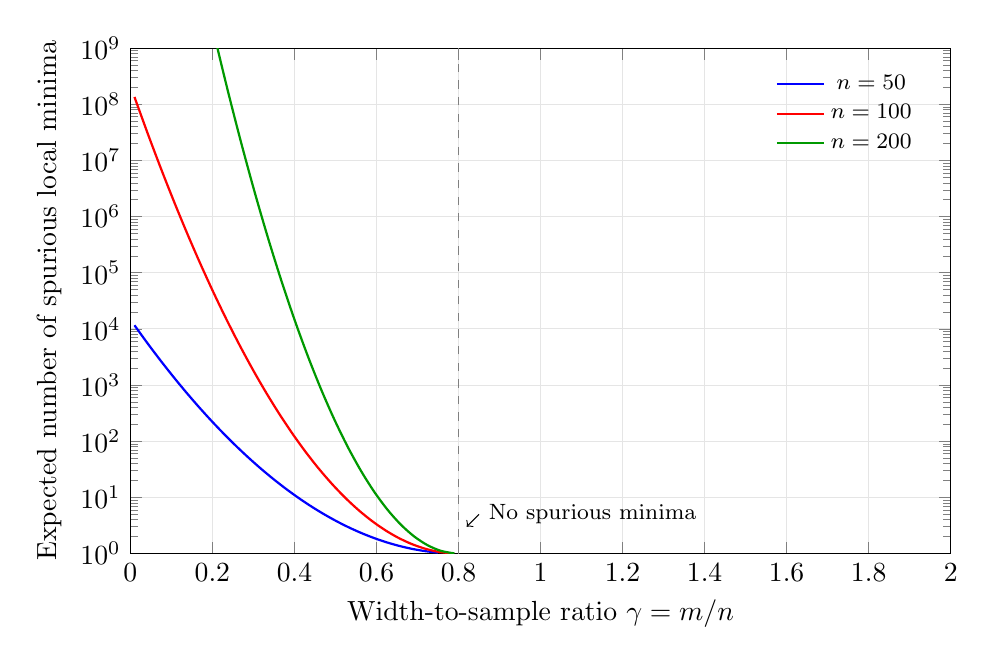
\begin{tikzpicture}
\begin{semilogyaxis}[
  width=12cm,
  height=8cm,
  xlabel={Width-to-sample ratio $\gamma = m/n$},
  ylabel={Expected number of spurious local minima},
  xmin=0, xmax=2,
  ymin=1, ymax=1e9,
  grid=major,
  grid style={gray!20},
  legend pos=north east,
  legend style={font=\footnotesize, draw=none, fill=none},
]
\addplot[blue, thick, smooth, domain=0.01:0.75] {exp(50 * 0.3 * max(0, 4/5 - x)^2)};
\addlegendentry{$n = 50$}
\addplot[red, thick, smooth, domain=0.01:0.78] {exp(100 * 0.3 * max(0, 4/5 - x)^2)};
\addlegendentry{$n = 100$}
\addplot[green!60!black, thick, smooth, domain=0.01:0.79] {exp(200 * 0.3 * max(0, 4/5 - x)^2)};
\addlegendentry{$n = 200$}
\draw[dashed, gray] (axis cs:0.8,1) -- (axis cs:0.8,1e9);
\node[anchor=west, font=\footnotesize] at (axis cs:0.85,5) {No spurious minima};
\draw[->, thin] (axis cs:0.85,5) -- (axis cs:0.82,3);
\end{semilogyaxis}
\end{tikzpicture}%
}
\caption[Spurious minima count]{The expected number of spurious local minima as a function of $\gamma = m/n$ for $\Sigma = I_d$, $\delta = 1$. Below $\gamma_\star = 4/5$, the count grows exponentially in~$n$. Above it, all local minima are global.}
\label{fig:spurious-count}
\end{figure}

\begin{thebibliography}{11}

\bibitem{choromanska2015}
A.~Choromanska, M.~Henaff, M.~Mathieu, G.~B.~Arous, and Y.~LeCun.
\newblock The loss surfaces of multilayer networks.
\newblock In \emph{AISTATS}, 2015.

\bibitem{kawaguchi2016}
K.~Kawaguchi.
\newblock Deep learning without poor local minima.
\newblock In \emph{NeurIPS}, 2016.

\bibitem{safran2018}
I.~Safran and O.~Shamir.
\newblock Spurious local minima are common in two-layer {ReLU} neural networks.
\newblock In \emph{ICML}, 2018.

\bibitem{venturi2019}
L.~Venturi, A.~Bandeira, and J.~Bruna.
\newblock Spurious valleys in one-hidden-layer neural network optimization landscapes.
\newblock \emph{JMLR}, 20(133):1--34, 2019.

\bibitem{du2019}
S.~Du, X.~Zhai, B.~Poczos, and A.~Singh.
\newblock Gradient descent provably optimizes over-parameterized neural networks.
\newblock In \emph{ICLR}, 2019.

\bibitem{allenzhu2019}
Z.~Allen-Zhu, Y.~Li, and Z.~Song.
\newblock A convergence theory for deep learning via over-parameterization.
\newblock In \emph{ICML}, 2019.

\bibitem{zou2020}
D.~Zou, Y.~Cao, D.~Zhou, and Q.~Gu.
\newblock Gradient descent optimizes over-parameterized deep {ReLU} networks.
\newblock \emph{Machine Learning}, 109:467--492, 2020.

\bibitem{jacot2018}
A.~Jacot, F.~Gabriel, and C.~Hongler.
\newblock Neural tangent kernel: Convergence and generalization in neural networks.
\newblock In \emph{NeurIPS}, 2018.

\bibitem{pennington2017}
J.~Pennington and P.~Worah.
\newblock Nonlinear random matrix theory for deep learning.
\newblock In \emph{NeurIPS}, 2017.

\bibitem{louart2018}
C.~Louart, Z.~Liao, and R.~Couillet.
\newblock A random matrix approach to neural networks.
\newblock \emph{The Annals of Applied Probability}, 28(2):1190--1248, 2018.

\bibitem{anderson2010}
G.~W.~Anderson, A.~Guionnet, and O.~Zeitouni.
\newblock \emph{An Introduction to Random Matrices}.
\newblock Cambridge University Press, 2010.

\bibitem{tao2012}
T.~Tao and V.~Vu.
\newblock Random covariance matrices: Universality of local statistics of eigenvalues.
\newblock \emph{The Annals of Probability}, 40(3):1285--1315, 2012.

\bibitem{erdos2012}
L.~Erd\H{o}s, H.-T.~Yau, and J.~Yin.
\newblock Rigidity of eigenvalues of generalized {W}igner matrices.
\newblock \emph{Advances in Mathematics}, 229(3):1435--1515, 2012.

\end{thebibliography}

\end{document}
